Per l'esecuzione del'esperienza è stato utilizzato il seguente apparato sperimentale:
\begin{itemize}
	\item Guida ottica
	\item Lente
	\item Sorgente luminosa (candela)
	\item Schermo
\end{itemize}

\begin{table}[H]
	\centering
	\begin{tabular}{|c|c|}
		\hline
		\textbf{Strumenti di misura} & \textbf{Risoluzione} \\
		\hline
		Guida ottica & $0.05\ cm$ \\
		\hline
	\end{tabular}
	\caption{Risoluzione degli strumenti di misura utilizzati}
	\label{tab:}
\end{table}

\begin{figure}[H]
	\centering
	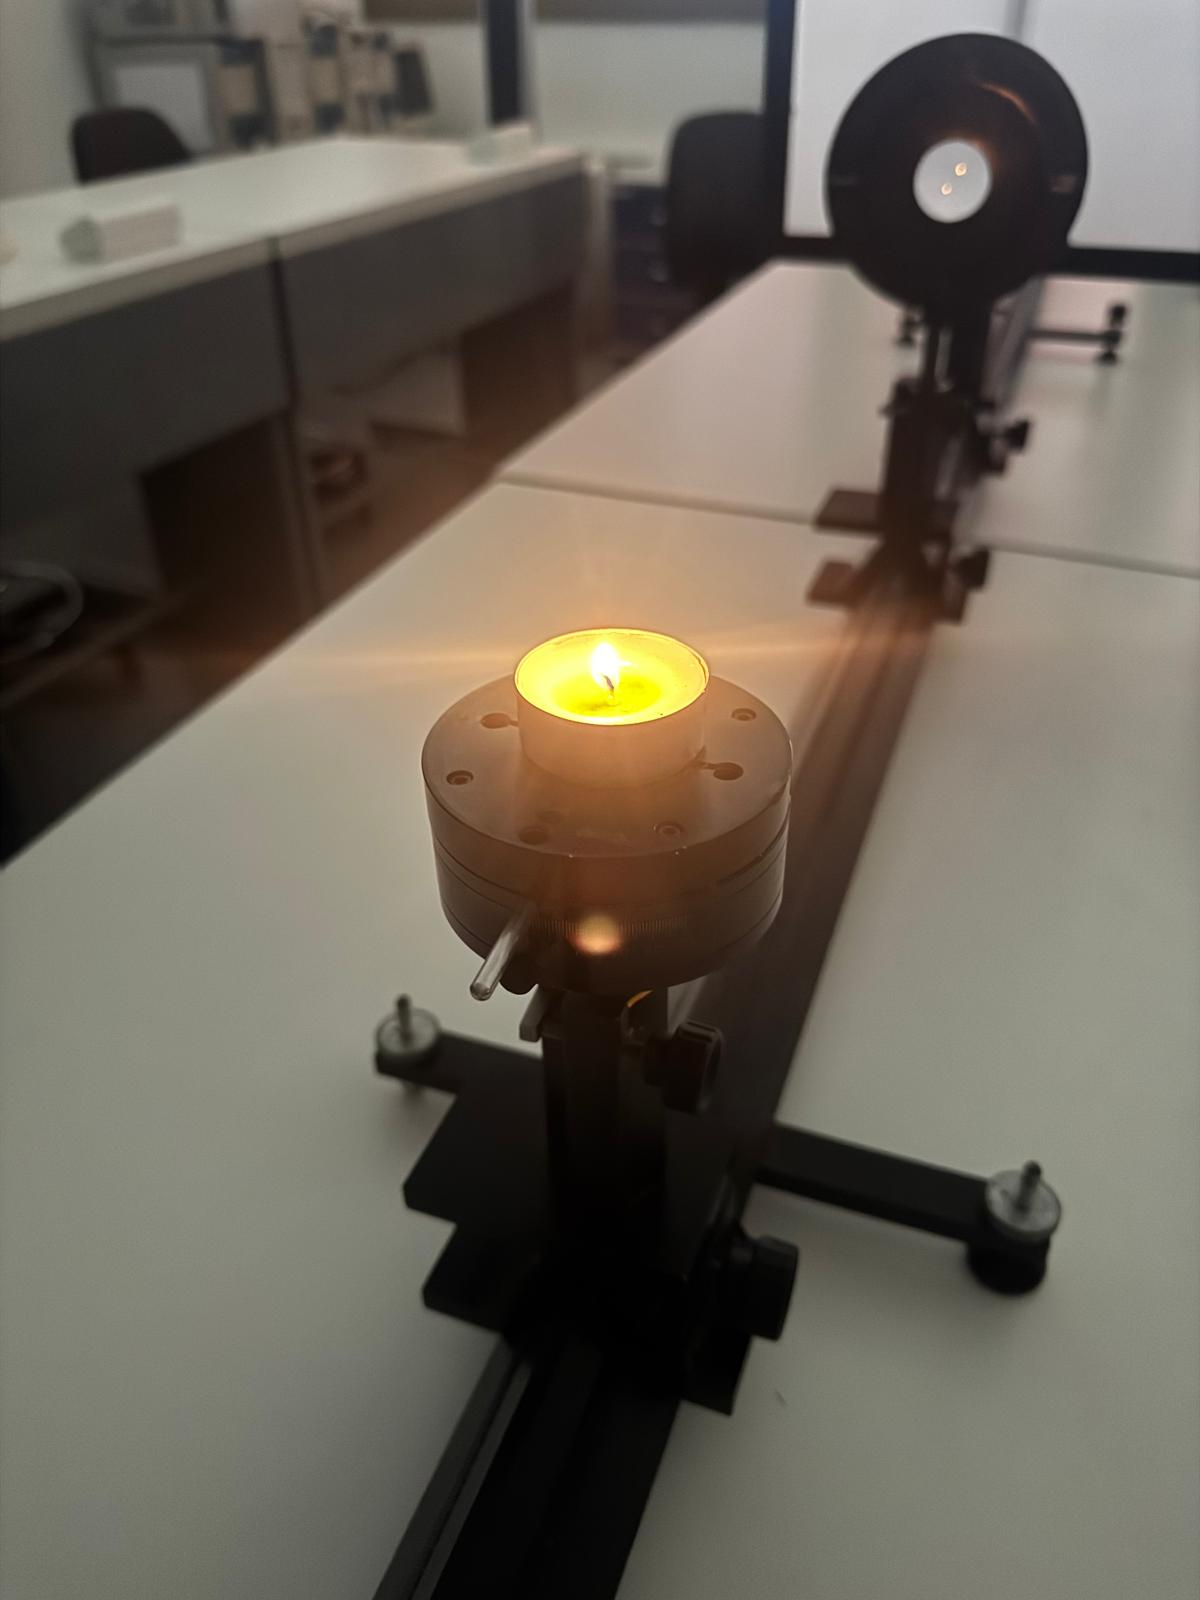
\includegraphics[width=0.4\textwidth]{./lucina}
	\caption{Candela utilizzata come fonte luminosa per l'esperimento.}
\end{figure}

\begin{figure}[H]
	\centering
	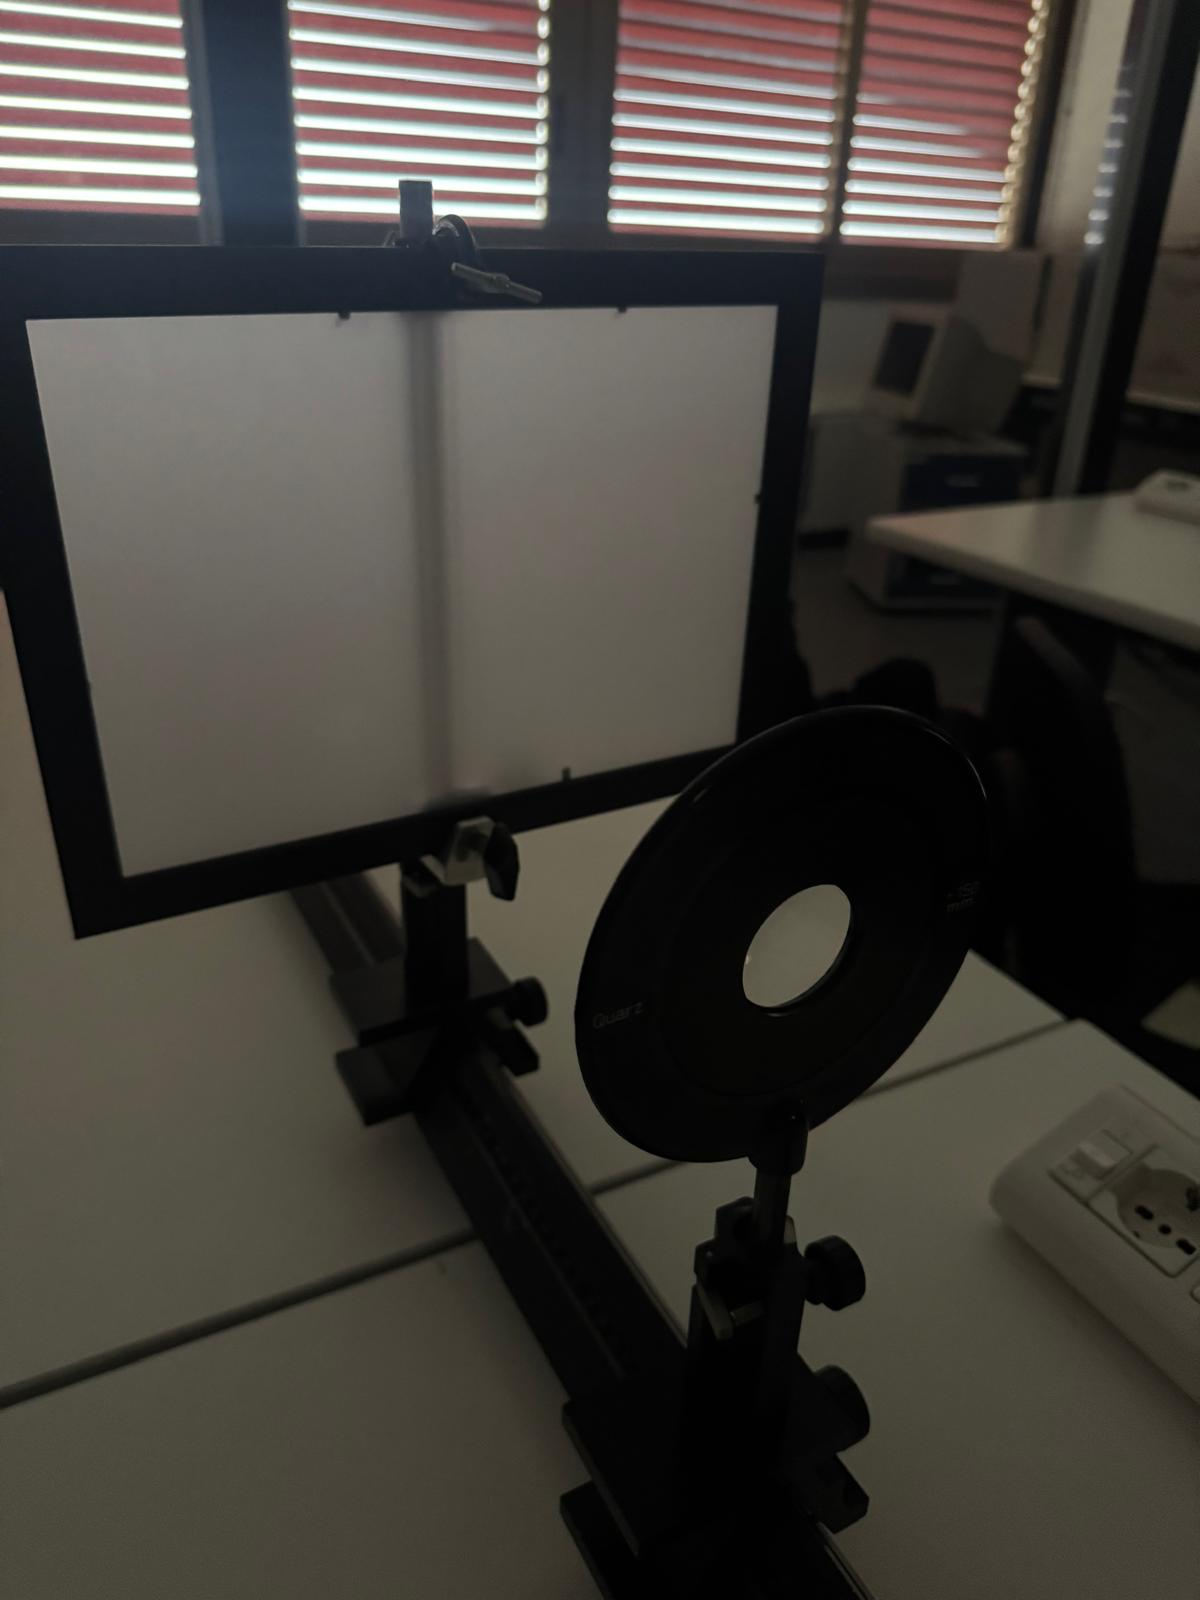
\includegraphics[width=0.4\textwidth]{./lente}
	\caption{Lente e schermo posizionati sulla guida ottica.}
\end{figure}